% Compile with: uplatex file.tex && dvipdfmx file.dvi
%           or: latexmk -uplatex file.tex
%\documentclass[uplatex,dvipdfmx]{jsarticle}
\documentclass[dvipdfmx,a4paper,11pt]{jsarticle}
\usepackage{amsmath, amssymb}
\usepackage{tikz}

\title{scenario\_lattice\_figures}
\date{\today}

\begin{document}
\maketitle

ハニカム格子（3$\times$3、開放境界）上で、隣接サイト対 $\langle ij\rangle$ にわたる和 $\sum_{\langle ij\rangle}S_i^zS_j^z$ を、実際のボンド（隣接ペア）に展開する。

$Sz_i$ $Sz_j$ のハニカム格子 3x3 の最近接和を展開して

\begin{equation}
  Sz\left(8\right) Sz\left(9\right)+Sz\left(7\right) Sz\left(8\right)+Sz\left(5\right) Sz\left(8\right)+Sz\left(5\right) Sz\left(6\right)+Sz\left(3\right) Sz\left(6\right)+Sz\left(4\right) Sz\left(5\right)+Sz\left(1\right) Sz\left(4\right)+Sz\left(2\right) Sz\left(3\right)+Sz\left(1\right) Sz\left(2\right)
  \label{eq:E1}
\end{equation}

\begin{center}
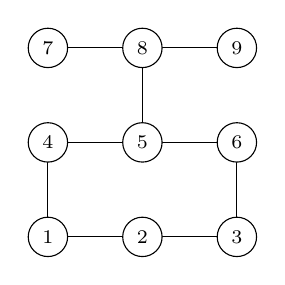
\begin{tikzpicture}[scale=1.2, site/.style={circle,draw,fill=white,inner sep=1pt,minimum size=5mm,font=\scriptsize}]
  \draw (0.000,0.000) -- (1.000,0.000);
  \draw (1.000,0.000) -- (2.000,0.000);
  \draw (0.000,1.000) -- (1.000,1.000);
  \draw (1.000,1.000) -- (2.000,1.000);
  \draw (0.000,2.000) -- (1.000,2.000);
  \draw (1.000,2.000) -- (2.000,2.000);
  \draw (0.000,0.000) -- (0.000,1.000);
  \draw (1.000,1.000) -- (1.000,2.000);
  \draw (2.000,0.000) -- (2.000,1.000);
  \node[site] at (0.000,0.000) {1};
  \node[site] at (1.000,0.000) {2};
  \node[site] at (2.000,0.000) {3};
  \node[site] at (0.000,1.000) {4};
  \node[site] at (1.000,1.000) {5};
  \node[site] at (2.000,1.000) {6};
  \node[site] at (0.000,2.000) {7};
  \node[site] at (1.000,2.000) {8};
  \node[site] at (2.000,2.000) {9};
\end{tikzpicture}
\end{center}

直前の格子和のボンド構造を図として保存する（SVGとスタンドアロンTeX、可能ならPDFも）。図を見ることで、意図した格子・境界条件になっているかを確認できる。

格子図を保存して

今度は正方格子（3$\times$3）で、周期境界条件のもとで同じ最近接和を展開する。周期境界により生じる端と端をつなぐボンドは、図では破線として区別される。

$Sz_i$ $Sz_j$ の正方格子 3x3 の周期境界で最近接和を展開して

\begin{equation}
  Sz\left(8\right) Sz\left(9\right)+Sz\left(7\right) Sz\left(9\right)+Sz\left(6\right) Sz\left(9\right)+Sz\left(3\right) Sz\left(9\right)+Sz\left(7\right) Sz\left(8\right)+Sz\left(5\right) Sz\left(8\right)+Sz\left(2\right) Sz\left(8\right)+Sz\left(4\right) Sz\left(7\right)+Sz\left(1\right) Sz\left(7\right)+Sz\left(5\right) Sz\left(6\right)+Sz\left(4\right) Sz\left(6\right)+Sz\left(3\right) Sz\left(6\right)+Sz\left(4\right) Sz\left(5\right)+Sz\left(2\right) Sz\left(5\right)+Sz\left(1\right) Sz\left(4\right)+Sz\left(2\right) Sz\left(3\right)+Sz\left(1\right) Sz\left(3\right)+Sz\left(1\right) Sz\left(2\right)
  \label{eq:E2}
\end{equation}

\begin{center}
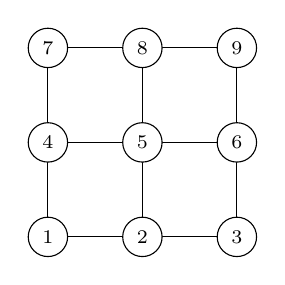
\begin{tikzpicture}[scale=1.2, site/.style={circle,draw,fill=white,inner sep=1pt,minimum size=5mm,font=\scriptsize}]
  \draw (0.000,0.000) -- (1.000,0.000);
  \draw (1.000,0.000) -- (2.000,0.000);
  \draw[dashed] (2.000,0.000) -- (0.000,0.000);
  \draw (0.000,1.000) -- (1.000,1.000);
  \draw (1.000,1.000) -- (2.000,1.000);
  \draw[dashed] (2.000,1.000) -- (0.000,1.000);
  \draw (0.000,2.000) -- (1.000,2.000);
  \draw (1.000,2.000) -- (2.000,2.000);
  \draw[dashed] (2.000,2.000) -- (0.000,2.000);
  \draw (0.000,0.000) -- (0.000,1.000);
  \draw (0.000,1.000) -- (0.000,2.000);
  \draw[dashed] (0.000,2.000) -- (0.000,0.000);
  \draw (1.000,0.000) -- (1.000,1.000);
  \draw (1.000,1.000) -- (1.000,2.000);
  \draw[dashed] (1.000,2.000) -- (1.000,0.000);
  \draw (2.000,0.000) -- (2.000,1.000);
  \draw (2.000,1.000) -- (2.000,2.000);
  \draw[dashed] (2.000,2.000) -- (2.000,0.000);
  \node[site] at (0.000,0.000) {1};
  \node[site] at (1.000,0.000) {2};
  \node[site] at (2.000,0.000) {3};
  \node[site] at (0.000,1.000) {4};
  \node[site] at (1.000,1.000) {5};
  \node[site] at (2.000,1.000) {6};
  \node[site] at (0.000,2.000) {7};
  \node[site] at (1.000,2.000) {8};
  \node[site] at (2.000,2.000) {9};
\end{tikzpicture}
\end{center}

\end{document}